\documentclass[a4paper,UTF8]{ctexart}

\usepackage{amsmath, amsthm, amssymb, amsfonts, hyperref, mathrsfs}%美国数学学会的包+?
\usepackage{geometry} %控制界面
\usepackage{bookmark}
\usepackage{fancyhdr} % header & footer
\usepackage{appendix} % 附录
\usepackage{tikz} %作图
\usepackage{graphicx} %插入图片的宏包
\usepackage{float} %设置图片浮动位置的宏包
%\usepackage{subfigure} %插入多图时用子图显示的宏包
\usepackage{listings} %引用代码
\usepackage{physics,mathtools} %物理数学工具
\usepackage{comment}
\usepackage{framed}
\usepackage{caption}
\usepackage{subcaption}
\geometry{top=2.5cm,bottom=2.5cm,left=2.5cm,right=2.5cm} % 布局要求
\pagestyle{fancy} % fancy分格
\fancyhf{} % 清除所有页眉页脚
\renewcommand\headrulewidth{0.6pt}
\renewcommand\footrulewidth{0.6pt}
% font
\setCJKmainfont{Noto Serif CJK SC}[BoldFont={Noto Serif CJK SC Bold}, ItalicFont=]
\lhead{何金铭 PB21020660$\mid$座位号:8}
\cfoot{纠缠光子的制备及性质实验报告}
\rhead{\thepage}
\lfoot{2024.4.28}
\rfoot{USTC}
%\bibliographystyle{plain} % 引用样式
\everymath{\displaystyle} % display
%============================================================

\begin{document}

\begin{center}
    \textbf{\Large 纠缠光子的制备及性质实验报告}
    \par \text{\large 何金铭 PB21020660}
\end{center}

实验目的,实验原理,实验内容已于预习报告中给出,这里不再复述。

\section{实验结果与分析}

\subsection{系统搭建1}

\begin{table}[H]
    \centering
    \caption{光子数计数表1}
    \begin{tabular}{|l|l|}
    \hline
        \textbf{偏振片组合} & \textbf{符合计数} \\ \hline
        0/90° & 3650 \\ \hline
        90°/0 & 2129 \\ \hline
    \end{tabular}
\end{table}

\begin{table}[H]
    \centering
    \caption{光子数计数表2}
    \begin{tabular}{|l|l|}
    \hline
        \textbf{偏振片组合} & \textbf{符合计数} \\ \hline
        45°/45° & 2564 \\ \hline
        -45°/-45° & 1716 \\ \hline
        45°/-45° & 51 \\ \hline
        -45°/45° & 53 \\ \hline
    \end{tabular}
\end{table}

\subsection{CHSH不等式的测量}

记:$\theta_{a1} = 0^{\circ},\theta_{a2} = 45^{\circ},\theta_{b1} = 22.5^{\circ},\theta_{b2} = -22.5^{\circ}$

\begin{table}[H]
    \centering
    \caption{CHSH不等式偏振组合1}
    \begin{tabular}{|l|l|}
    \hline
        \textbf{偏振片组合} & \textbf{符合计数} \\ \hline
        $C(\theta_{a1},\theta_{b1})$ & 304 \\ \hline
        $C(\theta_{a1},\theta_{b1}^{\bot})$ & 2466 \\ \hline
        $C(\theta_{a1}^{\bot},\theta_{b1})$ & 2180 \\ \hline
        $C(\theta_{a1}^{\bot},\theta_{b1}^{\bot})$ & 537 \\ \hline
    \end{tabular}
\end{table}

得:$E(a_1,b_1) = -0.6935$

\begin{table}[H]
    \centering
    \caption{CHSH不等式偏振组合2}
    \begin{tabular}{|l|l|}
    \hline
        \textbf{偏振片组合} & \textbf{符合计数} \\ \hline
        $C(\theta_{a1},\theta_{b2})$ & 164 \\ \hline
        $C(\theta_{a1},\theta_{b2}^{\bot})$ & 2056 \\ \hline
        $C(\theta_{a1}^{\bot},\theta_{b2})$ & 2167 \\ \hline
        $C(\theta_{a1}^{\bot},\theta_{b2}^{\bot})$ & 225 \\ \hline
    \end{tabular}
\end{table}

得: $E(a_1,b_2) = -0.8313$

\begin{table}[H]
    \centering
    \caption{CHSH不等式偏振组合3}
    \begin{tabular}{|l|l|}
    \hline
        \textbf{偏振片组合} & \textbf{符合计数} \\ \hline
        $C(\theta_{a2},\theta_{b1})$ & 2049 \\ \hline
        $C(\theta_{a2},\theta_{b1}^{\bot})$ & 356 \\ \hline
        $C(\theta_{a2}^{\bot},\theta_{b1})$ & 410 \\ \hline
        $C(\theta_{a1}^{\bot},\theta_{b1}^{\bot})$ & 2545 \\ \hline
    \end{tabular}
\end{table}

得: $E(a_2,b_1) = 0.7142$

\begin{table}[H]
    \centering
    \caption{CHSH不等式偏振组合4}
    \begin{tabular}{|l|l|}
    \hline
        \textbf{偏振片组合} & \textbf{符合计数} \\ \hline
        $C(\theta_{a2},\theta_{b2})$ & 550 \\ \hline
        $C(\theta_{a2},\theta_{b2}^{\bot})$ & 1928 \\ \hline
        $C(\theta_{a2}^{\bot},\theta_{b2})$ & 1719 \\ \hline
        $C(\theta_{a1}^{\bot},\theta_{b1}^{\bot})$ & 390 \\ \hline
    \end{tabular}
\end{table}

得: $E(a_2,b_2) = -0.5901$

最终计算得:

$$
|E\left(\boldsymbol{a}_1,\boldsymbol{b}_1\right)+E\left(\boldsymbol{a}_1,\boldsymbol{b}_2\right)+E\left(\boldsymbol{a}_2,\boldsymbol{b}_1\right)-E\left(\boldsymbol{a}_2,\boldsymbol{b}_2\right)| = 2.8291 = 2\sqrt{2} + 0.00067,
$$

CHSH不等式的误差在$0.5\%$以内,可以认为此结果为$2\sqrt{2}>2$违背了CHSH不等式。

\subsection{测量关联曲线}

\subsubsection{一个偏振片为$0^{\circ}$时的关联曲线}

\begin{table}[H]
    \centering
    \caption{一个偏振片为$0^{\circ}$时的关联曲线记录表}
    \begin{tabular}{|l|l|l|l|}
    \hline
        \textbf{转动角度} & \textbf{光子计数} & \textbf{转动角度} & \textbf{光子计数} \\ \hline
        0 & 333 & 100 & 2501 \\ \hline
        10 & 109 & 110 & 2417 \\ \hline
        20 & 338 & 120 & 2047 \\ \hline
        30 & 592 & 130 & 1602 \\ \hline
        40 & 952 & 140 & 1037 \\ \hline
        50 & 1401 & 150 & 666 \\ \hline
        60 & 1794 & 160 & 201 \\ \hline
        70 & 2134 & 170 & 32 \\ \hline
        80 & 2544 & 180 & 20 \\ \hline
    \end{tabular}
\end{table}

\begin{figure}[H]
    \centering
    \begin{minipage}[b]{0.9\textwidth}
        \centering
        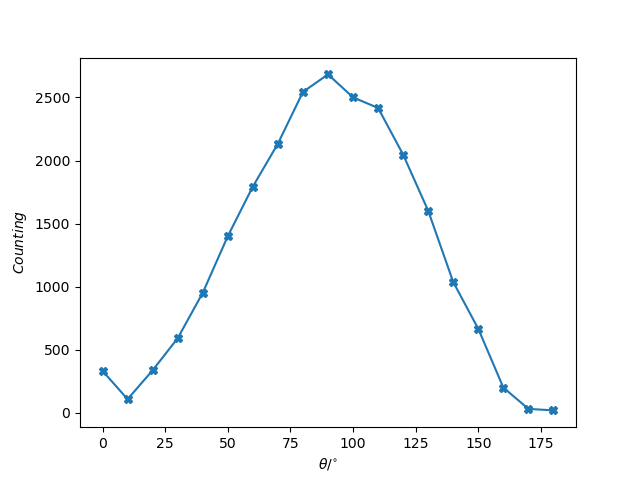
\includegraphics[width=0.9\textwidth]{./1.png}
        \caption{一个偏振片为$0^{\circ}$时的关联曲线}
        \label{1}
    \end{minipage}
\end{figure}

\subsubsection{一个偏振片为$45^{\circ}$时的关联曲线}

\begin{table}[H]
    \centering
    \caption{一个偏振片为$45^{\circ}$时的关联曲线记录表}
    \begin{tabular}{|l|l|l|l|}
    \hline
        \textbf{转动角度} & \textbf{光子计数} & \textbf{转动角度} & \textbf{光子计数} \\ \hline
        0 & 1416 & 100 & 807 \\ \hline
        10 & 1773 & 110 & 428 \\ \hline
        20 & 2036 & 120 & 228 \\ \hline
        30 & 2232 & 130 & 92 \\ \hline
        40 & 2307 & 140 & 41 \\ \hline
        50 & 2232 & 150 & 136 \\ \hline
        60 & 2060 & 160 & 338 \\ \hline
        70 & 1813 & 170 & 642 \\ \hline
        80 & 1441 & 180 & 922 \\ \hline
    \end{tabular}
\end{table}

\begin{figure}[H]
    \centering
    \begin{minipage}[b]{0.9\textwidth}
        \centering
        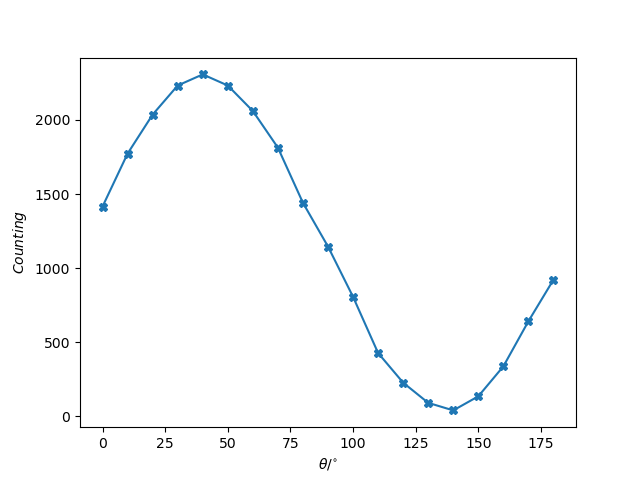
\includegraphics[width=0.9\textwidth]{./2.png}
        \caption{一个偏振片为$45^{\circ}$时的关联曲线}
        \label{2}
    \end{minipage}
\end{figure}

\section{实验结论}

\begin{enumerate}
    \item 取$\theta_{a1} = 0^{\circ},\theta_{a2} = 45^{\circ},\theta_{b1} = 22.5^{\circ},\theta_{b2} = -22.5^{\circ}$,测得结果违背了CHSH不等式
    \item 并且测得了一个偏振片角度为$0^{\circ},45^{\circ}$的结果,发现关联曲线有明显的干涉特性
\end{enumerate}

\section{思考题}

\subsection{实验原理部分给出的CHSH不等式最大违背条件下有$B_{\mathrm{CHSH}}=2\sqrt{2}$, 给出详细计算过程.}

取$\theta_{a1} = 0^{\circ},\theta_{a2} = 45^{\circ},\theta_{b1} = 22.5^{\circ},\theta_{b2} = -22.5^{\circ}$,
在Bloch矢量中,偏振片的角度$0^{\circ}$对应了$\ket{V}$, $22.5^{\circ}$对应了$\ket{+}$则有:

\begin{enumerate}
    \item $E(a_1,b_1) = - \cos(45^{\circ})$
    \item $E(a_1,b_2) = - \cos(45^{\circ})$
    \item $E(a_2,b_1) = - \cos(45^{\circ})$
    \item $E(a_2,b_2) = - \cos(135^{\circ})$
\end{enumerate}

$$
|E\left(\boldsymbol{a}_1,\boldsymbol{b}_1\right)+E\left(\boldsymbol{a}_1,\boldsymbol{b}_2\right)+E\left(\boldsymbol{a}_2,\boldsymbol{b}_1\right)-E\left(\boldsymbol{a}_2,\boldsymbol{b}_2\right)| = 2\sqrt{2}
$$

\subsection{根据实验数据分析,该实验中我们制备的纠缠态是四个Bell态中的哪一个?  (需给出分析的过程)}

是Bell态中的$\ket{\Psi^{+}} = \frac{1}{\sqrt{2}}(\ket{01}+\ket{10})$ 态

分析如下:

\begin{figure}[H]
    \centering
    \begin{minipage}[b]{0.9\textwidth}
        \centering
        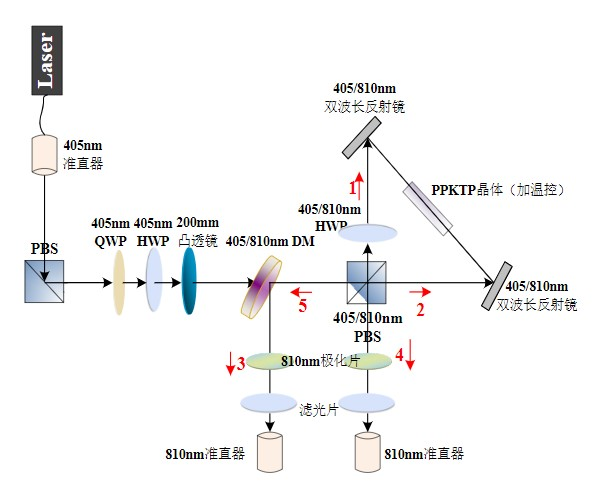
\includegraphics[width=0.9\textwidth]{./fig2.jpg}
        \caption{实验装置示意图}
    \end{minipage}
\end{figure}

 将 PPKTP 晶体和 Sagnac 环结合,即可产生高亮度的偏振纠缠源,下面给出详细分析. 
 泵浦光被由极化分束器(PBS)反射只剩下 V 分量,再由半波片将 V 极化的泵浦光置于 45°极化,
 之后再次入射极化分束器(PBS), H 分量透射,V 分量反射.透射部分直接进入 PPKTP 晶体,
 以一定概率打出一对信号光(H)和闲频光(V), 经 45 度半波片后极化翻转,分别记为
 $|V_s\rangle$和$|H_i\rangle$; 反射部分泵浦光经过 45 度半波片变换为 H, 
 同样以一定概率打出一对信号光(H)和闲频光(V), 分别记为$|H_s\rangle$和$|V_i\rangle$.
 透射和反射的泵浦光由于光强相同,所以泵出一对光子的概率也相同.
 透射(反射)泵浦光所产生的下转换光子分别沿Sagnac 环逆时针(顺指针)再次进入 PBS,
  经 PBS 变换,信号光进入路径 3, 闲频光进入路径 4, 记为
  $|V_s\rangle_3|H_i\rangle_4(|H_s\rangle_3|V_i\rangle_4)$.
  由于光子的全同性,当在 3 和 4 端口观测到符合计数时,我们无法分辨下转换光子的顺(逆)时针,
  此时在 3 和 4 路径上,两个光子便处于纠缠态

$$
|\Psi^{+}\rangle_{34}=\frac{1}{\sqrt{2}}\left(\left|V_{s}\right\rangle_{3}|H_{i}\rangle_{4}+\left|H_{s}\right\rangle_{3}|V_{i}\rangle_{4}\right).
$$ 

\subsection{实验中需调节405nm泵浦光路径上的四分之一波片和半波片,其作用是什么?}

作用为将入射的$\ket{V}$光转换为$\ket{+}$光使其既可以透过第二个PBS($\ket{H}$),也可以在第二个PBS上反射($\ket{V}$)

\subsection{如果我们实验中制备的态是HV和VH的概率叠加,测到的关联曲线会是什么样子?尝试计算此时CHSH不等式违背情况.结合本问题谈谈Sagnac环在实验中起到的作用.}

我们本次实验中制备的态就为HV和VH的概率叠加:

$$
|\Psi^{+}\rangle_{34}=\frac{1}{\sqrt{2}}\left(\left|V_{s}\right\rangle_{3}|H_{i}\rangle_{4}+\left|H_{s}\right\rangle_{3}|V_{i}\rangle_{4}\right).
$$

得到的关联曲线如图\ref{1},图\ref{2}所示。

Sagnac环的作用为:

\begin{enumerate}
    \item 进入路径 3(4)的光子均为信号(闲频)光,这样的Sagnac 结构能够避
免由于光谱不同产生的纠缠干涉对比度下降.
    \item  另外由于Sagnac 干涉环的两臂重合,故此结构能够保证即便较长距离的干涉,光子的波包也能较好的重合.
\end{enumerate}

\subsection{调研双光子干涉现象(Hong-Ou-Mandel  interference);该现象是由于光子的波色统计特性,如果用费米子做同样的实验会有怎样的现象. (选做)}

\subsubsection{HOM干涉的原理}

如下图所示,当两个光子沿路径a和b入射到分束器时,其出射光子的可能情况有四种,
即两个光子同时透射和反射,其中一个光子透射另一个光子反射,
分别对应下图中的四种光子出射分布情况。

\begin{figure}[H]
    \centering
    \begin{minipage}[b]{0.9\textwidth}
        \centering
        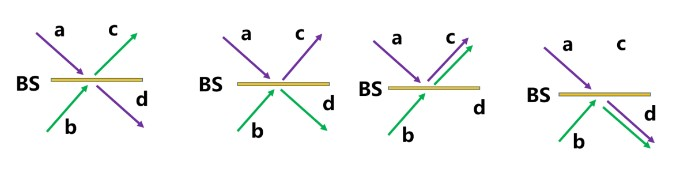
\includegraphics[width=0.9\textwidth]{./fig22.jpg}
        \caption{两光子入射到分束器上有四种可能的输出状态}
    \end{minipage}
\end{figure}

在光子数表象下,出射光子的量子态可以写成:

\begin{equation}
    \ket{\Phi}_{out} = (R-T) \ket{1_c,1_d} + i\sqrt{2RT}\ket{2_c,0_d} + \ket{0_c,2_d}
\end{equation}

其中{\bfseries{符合计数}}指:{\bfseries{c,d同时有光子出射}}

若假设我们的干涉滤波器的滤波函数是高斯型函数$g(\tau) = \exp{(-\Delta \omega \tau^2 /2)}$。最后得到复合计数的表达式为:

\begin{equation}
    N_{cd} = \kappa (T^2+R^2)[1-\frac{2RT}{T^2+R^2}\exp{(-\Delta \omega \delta \tau)}]
\end{equation}

可以很明显的看出,复合计数在相对延迟为零时的符合计数最低,形成一个低谷,低谷的半高宽度与光子的带宽$\Delta \omega$有关。
得到的结果如下图所示:

\begin{figure}[H]
    \centering
    \begin{minipage}[b]{0.9\textwidth}
        \centering
        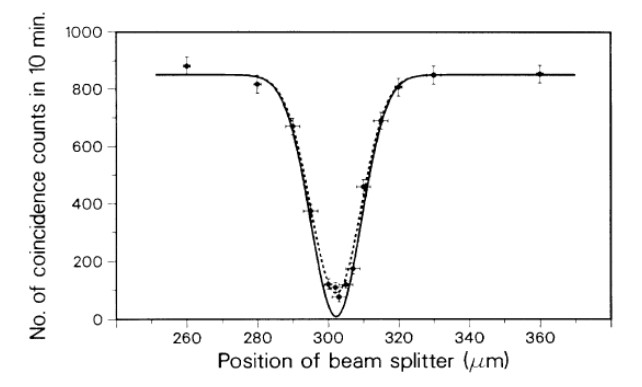
\includegraphics[width=0.9\textwidth]{./fig3.jpg}
        \caption{第一次HOM干涉曲线}
    \end{minipage}
\end{figure}

\subsubsection{费米子的HOM干涉}

然而,对于费米子(如电子),根据泡利不相容原理,两个费米子不能占据相同的量子态。因此,费米子的HOM干涉实验会有所不同。由于费米子的波函数是反对称的,两个费米子的波函数在空间上有所重叠时,它们的自旋或其他自由度必须不同,以满足泡利不相容原理。因此,费米子的HOM实验中,即使两个费米子的波包完全重叠,它们也不会产生完全的干涉,而是会出现一些分离。

因此,费米子的HOM干涉实验不会呈现出明显的干涉消除现象,而是会有一些衰减。这是由于费米子的反对称性质所导致的,与玻色子的干涉实验有所不同。

\end{document}